\begin{pages}
    \begin{Rightside}
    \selectlanguage{greek}
        \beginnumbering
        \pstart[
        			\chapter{Τὸ ἀρνίον ἀνοίγει τὸ βιβλίον}
        			\markboth{The Lamb Opens the Book}
				]
		\renewcommand{\LettrineFontHook}{\PHtitl}
		\lettrine[lines=3]{Κ}{αὶ} εἶδον ὅτε ἤνοιξεν τὸ Ἀρνίον μίαν ἐκ τῶν ἑπτὰ σφραγίδων, καὶ ἤκουσα ἑνὸς ἐκ τῶν τεσσάρων ζῴων λέγοντος ὡς φωνῇ βροντῆς Ἔρχου. καὶ εἶδον, καὶ ἰδοὺ ἵππος λευκός, καὶ ὁ καθήμενος ἐπ’ αὐτὸν ἔχων τόξον, καὶ ἐδόθη αὐτῷ στέφανος, καὶ ἐξῆλθεν νικῶν καὶ ἵνα νικήσῃ.
		\pend
		\pstart
		Καὶ ὅτε ἤνοιξεν τὴν σφραγῖδα τὴν δευτέραν, ἤκουσα τοῦ δευτέρου ζῴου λέγοντος Ἔρχου. καὶ ἐξῆλθεν ἄλλος ἵππος πυρρός, καὶ τῷ καθημένῳ ἐπ’ αὐτὸν ἐδόθη αὐτῷ λαβεῖν τὴν εἰρήνην ἐκ τῆς γῆς καὶ ἵνα ἀλλήλους σφάξουσιν, καὶ ἐδόθη αὐτῷ μάχαιρα μεγάλη.
		\pend
		\pstart
		Καὶ ὅτε ἤνοιξεν τὴν σφραγῖδα τὴν τρίτην, ἤκουσα τοῦ τρίτου ζῴου λέγοντος Ἔρχου. καὶ εἶδον, καὶ ἰδοὺ ἵππος μέλας, καὶ ὁ καθήμενος ἐπ’ αὐτὸν ἔχων ζυγὸν ἐν τῇ χειρὶ αὐτοῦ. καὶ ἤκουσα ὡς φωνὴν ἐν μέσῳ τῶν τεσσάρων ζῴων λέγουσαν Χοῖνιξ σίτου δηναρίου, καὶ τρεῖς χοίνικες κριθῶν δηναρίου· καὶ τὸ ἔλαιον καὶ τὸν οἶνον μὴ ἀδικήσῃς. 
		\pend
		\pstart
		Καὶ ὅτε ἤνοιξεν τὴν σφραγῖδα τὴν τετάρτην, ἤκουσα φωνὴν τοῦ τετάρτου ζῴου λέγοντος Ἔρχου. καὶ εἶδον, καὶ ἰδοὺ ἵππος χλωρός, καὶ ὁ καθήμενος ἐπάνω αὐτοῦ, ὄνομα αὐτῷ Ὁ Θάνατος, καὶ ὁ Ἅιδης ἠκολούθει μετ’ αὐτοῦ, καὶ ἐδόθη αὐτοῖς ἐξουσία ἐπὶ τὸ τέταρτον τῆς γῆς, ἀποκτεῖναι ἐν ῥομφαίᾳ καὶ ἐν λιμῷ καὶ ἐν θανάτῳ καὶ ὑπὸ τῶν θηρίων τῆς γῆς.
		\pend
		\pstart
		Καὶ ὅτε ἤνοιξεν τὴν πέμπτην σφραγῖδα, εἶδον ὑποκάτω τοῦ θυσιαστηρίου τὰς ψυχὰς τῶν ἐσφαγμένων διὰ τὸν λόγον τοῦ Θεοῦ καὶ διὰ τὴν μαρτυρίαν ἣν εἶχον. καὶ ἔκραξαν φωνῇ μεγάλῃ λέγοντες Ἕως πότε, ὁ Δεσπότης ὁ ἅγιος καὶ ἀληθινός, οὐ κρίνεις καὶ ἐκδικεῖς τὸ αἷμα ἡμῶν ἐκ τῶν κατοικούντων ἐπὶ τῆς γῆς; καὶ ἐδόθη αὐτοῖς ἑκάστῳ στολὴ λευκή, καὶ ἐρρέθη αὐτοῖς ἵνα ἀναπαύσωνται ἔτι χρόνον μικρόν, ἕως πληρωθῶσιν καὶ οἱ σύνδουλοι αὐτῶν καὶ οἱ ἀδελφοὶ αὐτῶν οἱ μέλλοντες ἀποκτέννεσθαι ὡς καὶ αὐτοί.
		\pend
		\pstart
		Καὶ εἶδον ὅτε ἤνοιξεν τὴν σφραγῖδα τὴν ἕκτην, καὶ σεισμὸς μέγας ἐγένετο, καὶ ὁ ἥλιος ἐγένετο μέλας ὡς σάκκος τρίχινος, καὶ ἡ σελήνη ὅλη ἐγένετο ὡς αἷμα, καὶ οἱ ἀστέρες τοῦ οὐρανοῦ ἔπεσαν εἰς τὴν γῆν, ὡς συκῆ βάλλει τοὺς ὀλύνθους αὐτῆς ὑπὸ ἀνέμου μεγάλου σειομένη, καὶ ὁ οὐρανὸς ἀπεχωρίσθη ὡς βιβλίον ἑλισσόμενον, καὶ πᾶν ὄρος καὶ νῆσος ἐκ τῶν τόπων αὐτῶν ἐκινήθησαν. 
		\pend
		\pstart
		καὶ οἱ βασιλεῖς τῆς γῆς καὶ οἱ μεγιστᾶνες καὶ οἱ χιλίαρχοι καὶ οἱ πλούσιοι καὶ οἱ ἰσχυροὶ καὶ πᾶς δοῦλος καὶ ἐλεύθερος ἔκρυψαν ἑαυτοὺς εἰς τὰ σπήλαια καὶ εἰς τὰς πέτρας τῶν ὀρέων, καὶ λέγουσιν τοῖς ὄρεσιν καὶ ταῖς πέτραις Πέσετε ἐφ’ ἡμᾶς καὶ κρύψατε ἡμᾶς ἀπὸ προσώπου τοῦ καθημένου ἐπὶ τοῦ θρόνου καὶ ἀπὸ τῆς ὀργῆς τοῦ Ἀρνίου, ὅτι ἦλθεν ἡ ἡμέρα ἡ μεγάλη τῆς ὀργῆς αὐτῶν, καὶ τίς δύναται σταθῆναι;
		\pend
        \endnumbering
    \end{Rightside}
    \begin{Leftside}
        \beginnumbering
        \pstart[
        			\chapter{The Lamb Opens the Book}
				]
		\renewcommand{\LettrineFontHook}{\Zallmanfamily}
		\lettrine[lines=3]{A}{nd} I saw when the Lamb opened one of the seals and I heard one of the four creatures saying in a thunderous voice, “Come.” And I saw — and look! — a white horse and he who sits upon it has a bow, and a crown was given to him and he departed victorious and to be victorious.
		\pend
		\pstart
		And when He (It, the Lamb) opened the second seal I heard the second creature saying, “Come.” And there came forth another fiery (having the colour of fire) horse, and to the one sitting upon it was given (the authority) to take the peace from the Earth so that they (the inhabitants of Earth) would slay each other and a great sword was given to him.
		\pend
		\pstart
		And when He opened the third seal, I heard the third creature saying, “Come.” And I saw — and look! — a great horse and he who sits upon it has a scale in his hand. And I heard (as) a voice in the middle of the four creatures saying, “A measure of wheat for a denarius (penny / cent \rightarrow\ small coin) and three measures of barley for a denarius; and do not mistreat the olive oil or the wine.”
		\pend
		\pstart
		And when He opened the fourth seal, I heard the voice of the fourth creature saying, “Come.” And I saw — and look! — a pale green (greenish-yellow) horse and the name of him who sits above (atop, on top of) it is (the) Death; and (the) Hades (Hell) follows (with) him; and power was given to them over a quarter of the Earth, to kill with sword and with hunger and with death and by (using) the beasts of the Earth.
		\pend
		\pstart
		And when He opened the fifth seal, I saw below the altar the souls of those who were slain because of the word of God and because of the testimony which they had. And they shouted in a loud voice saying, “Until when, O holy and true Master, will you not judge and vindicate our blood on the inhabitants of the Earth?” And to each of them was given a white robe and it was said to them (and they were told?) to rest for (yet) a little while until even (the number of) their fellow servants and their brothers — those who will be killed just as them — might be fulfilled (completed).
		\pend
		\pstart
		And I saw when He opened the sixth seal and a great tremor occurred; and the Sun became (as) black as a sackcloth (made out) of hair; and the entire moon became (in appearance) like blood and the stars of Heaven fell into (down onto) the Earth, just like a fig-tree throws its unripe fruit when shaken by a mighty storm (wind); and the sky was split apart like a book (scroll) being unrolled, and every mountain and island was moved from its place.
		\pend
		\pstart
		And the kings of the Earth and the noblemen, military commanders, the rich and strong and every slave and free man — (they all) hid themselves in caves and in (behind? under?) the stones of the mountains; and they say to the mountains and (to) the stones, “Fall upon us and hide us from the face of Him who sits upon the throne and (hide, protect) us from the Lamb’s wrath; for the great day of their wrath has come, and who shall be able to stand?”
		\pend
        \endnumbering
    \end{Leftside}

\end{pages} 
\Pages

\clearpage
\thispagestyle{empty}
\null\vfill
\settowidth\longest{\huge\itshape […] and when I turned around I saw}
\begin{center}
\parbox{\longest}{%
  \raggedright{\huge\itshape%
    ``And there came forth another fiery horse, and to the one sitting upon it was given (the authority) to take the peace from the Earth […]'' \par\bigskip
  }
  \raggedleft\Large\MakeUppercase{``Drie apocalyptische ruiters'' — Willem Adolfs, 1943}\par%
}
\vfill\vfill
\clearpage\newpage
\end{center}
\newpage
\thispagestyle{empty}
\begin{center}
	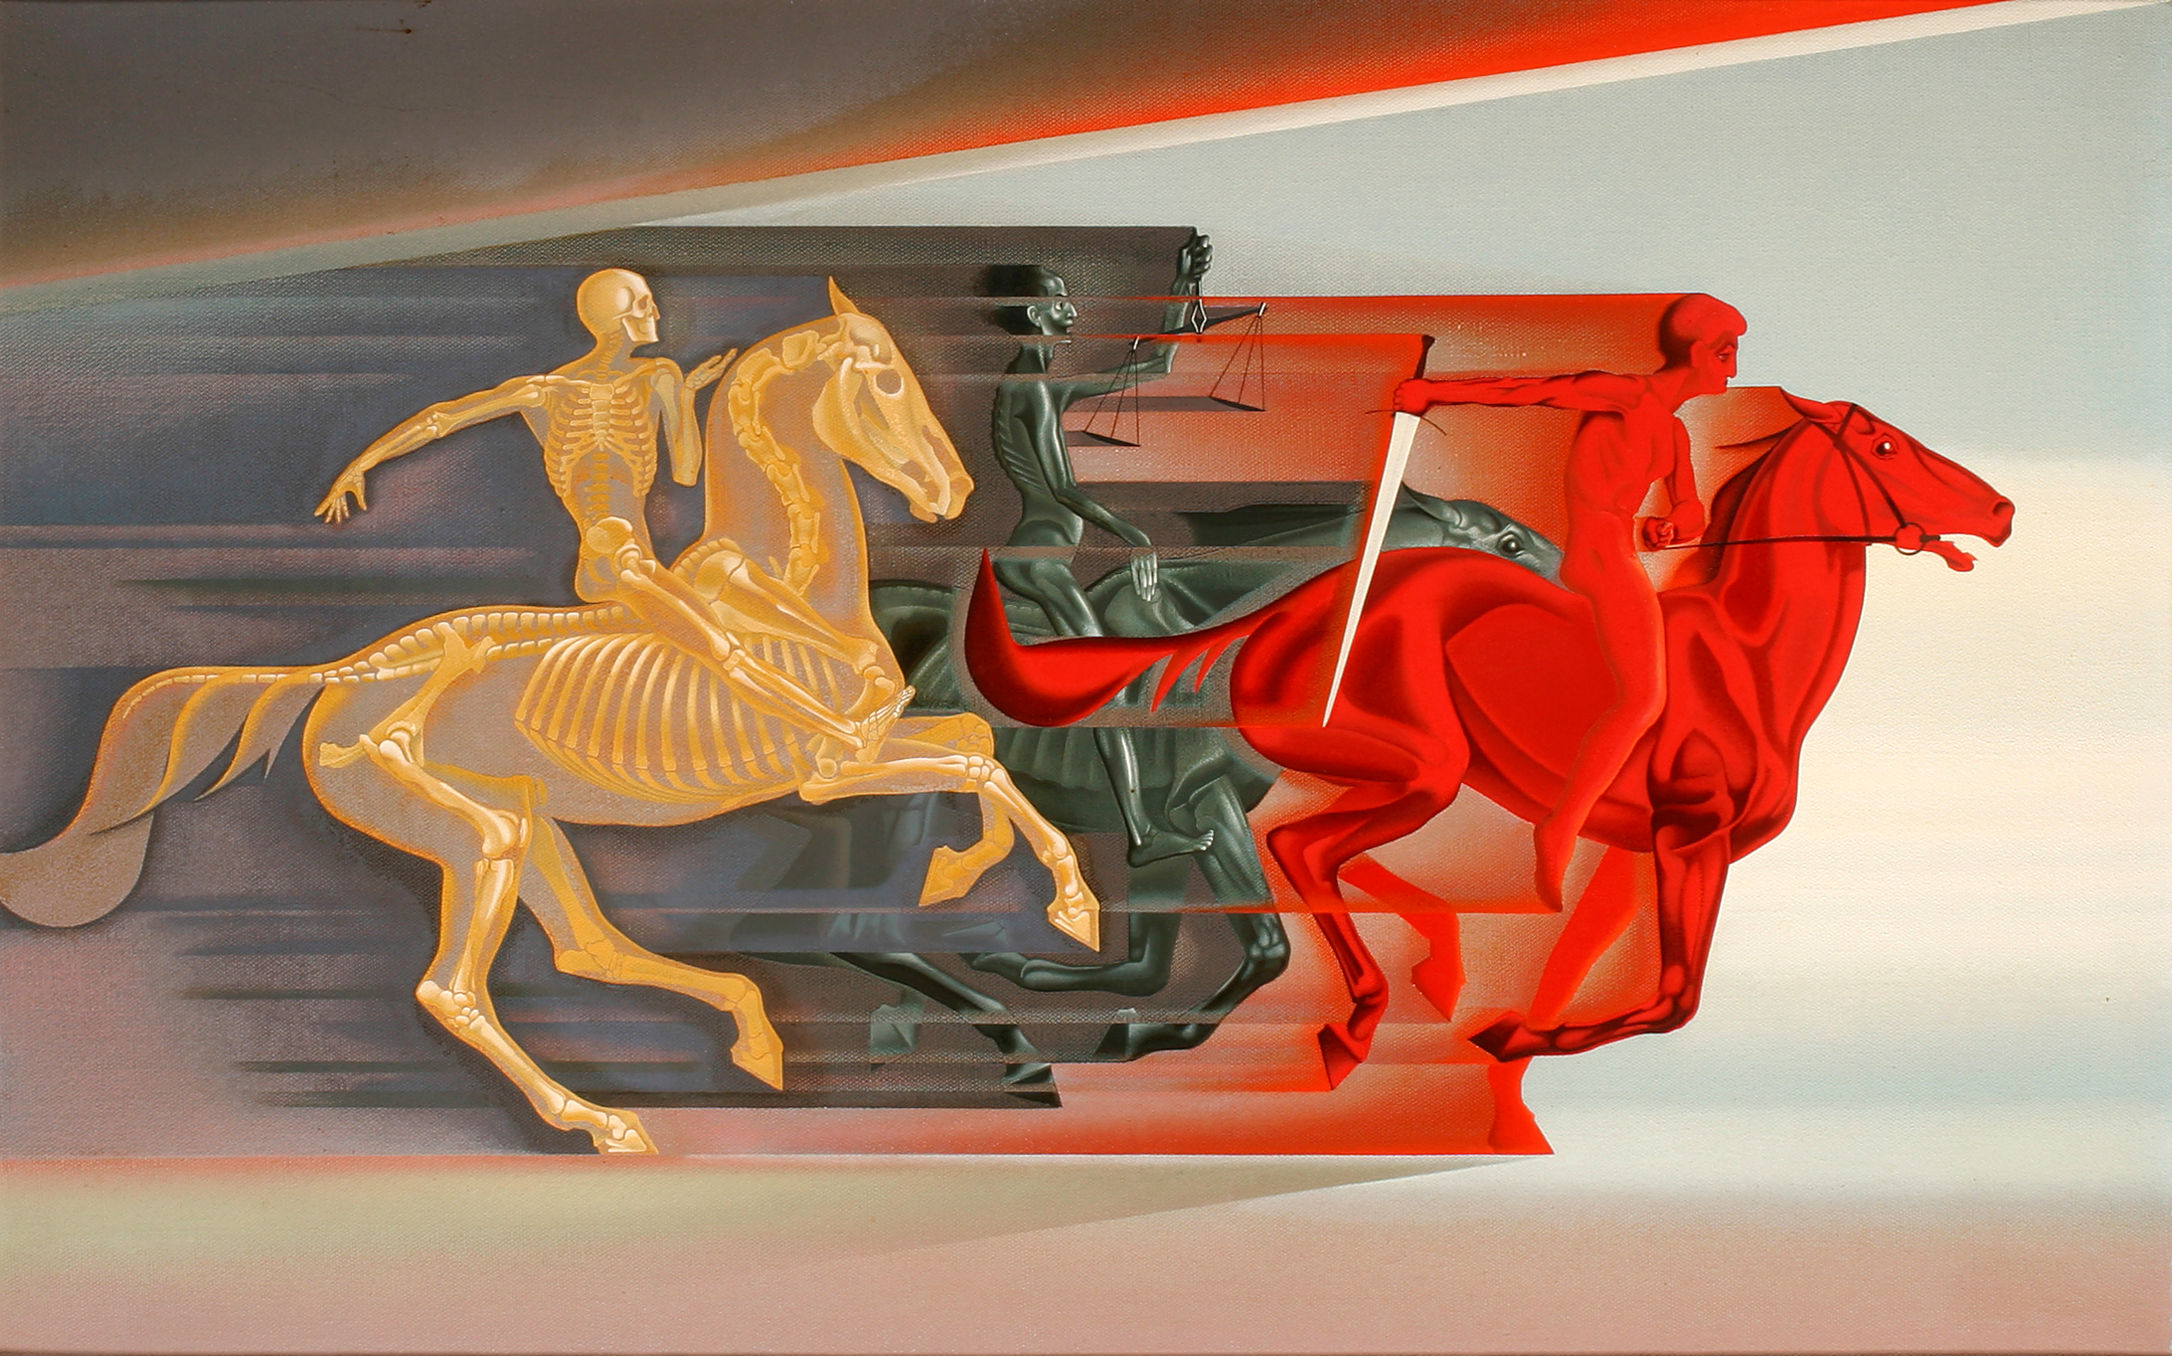
\includegraphics[angle=90, width=0.92\textwidth]{images/illustrations/adolfshorsemen.jpg}
\end{center}